\documentclass[11pt]{article}
\usepackage[margin=1in]{geometry}
\usepackage{amsmath,amssymb,bm}
\usepackage{booktabs,tabularx,array}
\usepackage{graphicx}
\usepackage{xcolor}
\usepackage[hyphens]{url}
\usepackage{hyperref}
\newcolumntype{Y}{>{\raggedright\arraybackslash}X}
\sloppy

\makeatletter
\newcommand{\code}[1]{{\def\_{\char`\_\discretionary{}{}{}}\texttt{#1}}}
\makeatother
\newcommand{\bq}{\mathbf{q}}
\newcommand{\bF}{\mathbf{F}}
\newcommand{\bS}{\mathbf{S}}
\newcommand{\bR}{\mathbf{R}}
\newcommand{\bu}{\mathbf{u}}
\newcommand{\dd}{\,\mathrm{d}}
\newcommand{\DSS}{\bigwedge_{e=1}^{N_e}}

\title{Reduced-gravity double gyre in \textsc{Jexpresso}:\\
\large equations, shallow-water limiter, and the entrainment floor}
\author{}
\date{November 2026}

\begin{document}
\maketitle

\noindent Case \code{problems/ShallowWater/ReducedGravity\_entrain}: the
\code{ReducedGravity} deck (wind-driven double gyre, after Choi et al.\ 2004)
plus the thin-layer treatment of Section~\ref{sec:floor}. CG spectral elements,
SSPRK54. This note describes what the code does; numbers quoted for the
standalone clone are from \code{tools/reduced\_gravity\_clone}.

%======================================================================
\section{Governing equations}
\label{sec:eqs}

One active layer of thickness $H(\mathbf{x},t)$ over a deep, motionless layer
(1.5-layer, reduced gravity $g'$), flat bottom, $\beta$-plane, closed basin
$\Omega=[0,L]^2$. In the flux form used by \textsc{Jexpresso},
\begin{equation}
\frac{\partial \bq}{\partial t} + \frac{\partial \bF}{\partial x}
+ \frac{\partial \mathbf{G}}{\partial y}
= \bS(\bq) + \nabla\cdot\left(\bm{\mu}\,\nabla\hat{\bq}\right),
\label{eq:pde}
\end{equation}
with the conserved variables, fluxes and sources (TOTAL form)
\begin{equation}
\bq=\begin{pmatrix} H\\ Hu\\ Hv\end{pmatrix},\quad
\bF=\begin{pmatrix} Hu\\ Hu^2+p\\ Huv\end{pmatrix},\quad
\mathbf{G}=\begin{pmatrix} Hv\\ Huv\\ Hv^2+p\end{pmatrix},
\label{eq:flux}
\end{equation}
\begin{equation}
\bS=\begin{pmatrix}
w_e(H)-\bar w\\
\phantom{-}f\,Hv+\alpha(H)\,\tau_x/\rho_0-\left[\kappa+\sigma(H)\right]Hu\\
-f\,Hu+\alpha(H)\,\tau_y/\rho_0-\left[\kappa+\sigma(H)\right]Hv
\end{pmatrix},
\label{eq:source}
\end{equation}
and $\hat{\bq}=(H-H_0,\,Hu,\,Hv)^{\mathsf T}$, $\bm{\mu}=\mathrm{diag}(0,\mu,\mu)$
(Laplacian artificial viscosity on the momenta only).
\begin{itemize}\setlength\itemsep{2pt}
\item \emph{Pressure.} $p=\tfrac12 g'(H^2-H_0^2)$, the perturbation about the
lake at rest $\bq_e=(H_0,0,0)^{\mathsf T}$ (\code{qe}); $\nabla p=g'H\nabla H$.
The well-balanced split of the island cases, here with $\nabla H_b=0$, so the
bathymetry source $-g'(H-H_0)\nabla H_b$ vanishes.
\item \emph{Velocity.} Fluxes use $H\leftarrow\max(H,0)$ and the
desingularized velocity (Kurganov \& Petrova 2007)
$u=\sqrt2\,H\,(Hu)/\sqrt{H^4+\max(H,\varepsilon)^4}$, equal to $Hu/H$ for
$H\ge\varepsilon=1$\,mm.
\item \emph{Forcing.} $f=f_0+\beta(y-L/2)$;
$\tau_x=-\tau_0\cos(2\pi y/L)$, $\tau_y=0$, weighted by the smoothstep
$\alpha(H)\in[0,1]$, $0$ for $H\le\varepsilon$ and $1$ for $H\ge 0.1$\,m;
linear drag $\kappa$; thin-film momentum relaxation
$\sigma(H)=\left[1-\alpha(H)\right]\sigma_0$.
\item \emph{Entrainment} from the deep layer, the floor of
Section~\ref{sec:floor} (McCreary \& Kundu 1988):
$w_e(H)=(H_e-H)^2/(t_eH_e)$ for $H<H_e$, $0$ otherwise; $\bar w$ is its basin
mean, removed by the volume compensation (Section~\ref{sec:comp}).
\end{itemize}

\begin{center}\small
\begin{tabular}{@{}llll@{}}
\toprule
$g'$ & $0.015$ m s$^{-2}$ & $H_0$ & $150$ m\\
$f_0$, $\beta$ & $8.37\times10^{-5}$ s$^{-1}$, $1.8\times10^{-11}$ m$^{-1}$s$^{-1}$ & $L$ & $2000$ km\\
$\tau_0$, $\rho_0$ & $0.03$ N m$^{-2}$, $1000$ kg m$^{-3}$ & $\kappa$ & $10^{-8}$ s$^{-1}$\\
$\sigma_0$ & $0.25/1200$ s$^{-1}$ & $\mu$ & $300$ m$^2$ s$^{-1}$\\
$H_e$, $t_e$ & $10$ m, $1$ day & $\varepsilon=h_{\min}$ & $10^{-3}$ m\\
\bottomrule
\end{tabular}
\end{center}

\paragraph{Discretization.} CG spectral elements of order $N=4$ on LGL
points, $25\times25$ quadrilaterals ($\Delta x_e=80$\,km, smallest LGL spacing
$\Delta x_{\min}=13.8$\,km), inexact (collocated) LGL integration, hence a
diagonal mass matrix $\mathbf{M}$. The inviscid terms are in strong form, the
viscous term in weak form, and the element contributions are assembled by
direct stiffness summation (DSS, $\bigwedge$):
\begin{equation}
\mathbf{M}\frac{\dd\bq}{\dd t}=\bR(\bq),\qquad
\bR=\DSS\Big[\mathbf{M}^{(e)}\big(\bS-\nabla\cdot\bF\big)^{(e)}
-\mathbf{L}^{(e)}_{\mu}\,\hat{\bq}^{(e)}\Big],
\label{eq:semi}
\end{equation}
with $\mathbf{M}^{(e)}_{ij}=\omega_i|J_i|\delta_{ij}$ and
$\mathbf{L}^{(e)}_\mu$ the element Laplacian. Free-slip walls are imposed
strongly ($\bu\cdot\mathbf{n}=0$ at boundary nodes). A Boyd--Vandeven (erf-log)
modal filter (Vandeven 1991), $\mathcal{F}=\mu_f\mathcal{F}_{\rm modal}+(1-\mu_f)\mathcal{I}$
with $\mu_f=0.05$ and modal weights $(1,1,1,0.996,0)$, acts on $\bq-\bq_e$
element by element and is projected back with $\mathbf{M}^{-1}\DSS$.
Time integration: SSPRK54 (Spiteri \& Ruuth 2002), $\Delta t=600$\,s
(gravity-wave Courant number $\approx0.12$).

%======================================================================
\section{The shallow-water limiter: what, where, when}
\label{sec:limiter}

\code{:swe\_limiter => "clip"}, \code{:swe\_limiter\_schedule => "stage"}
(\code{src/kernel/physics/shallow\_water\_limiter.jl}). Node by node:
\begin{enumerate}\setlength\itemsep{2pt}
\item \emph{Depth floor (clip).} If $H_i<h_{\min}$: $H_i\leftarrow h_{\min}$,
$(Hu)_i\leftarrow0$, $(Hv)_i\leftarrow0$. Not conservative: it adds
$\sum_iM_i(h_{\min}-H_i)$ of volume.
\item \emph{Velocity cap} (\code{:swe\_umax} $=u_{\max}>0$). If
$|(H\bu)_i|>u_{\max}H_i$: $(H\bu)_i\leftarrow u_{\max}H_i\,(H\bu)_i/|(H\bu)_i|$,
with $H_i$ unchanged, so mass is conserved. This is the shallow-water
counterpart of the momentum rescaling of the MHD realizability repair
(\code{src/kernel/positivity}): the derived quantity kept admissible is the
velocity $u=Hu/H$ instead of the pressure. In this case $u_{\max}=2$\,m\,s$^{-1}$
($\approx2.5\times$ the fastest physical flow, $\Delta x_{\min}/\Delta t/10$).
\end{enumerate}
It is the \emph{stage limiter} of the integrator, i.e.\ it acts on the
\emph{state}, not inside the right-hand side: it is applied to each of the
five SSPRK54 stage values, $\bq^{n+1}$ included, right after its Shu--Osher
update and before the next RHS evaluation, and once to the initial or restart
state. One step from $t^n$ reads
\begin{center}
\fbox{\parbox{0.92\textwidth}{\small
$\bq^{(0)}=\bq^n$;\quad for $s=1,\dots,5$:
\begin{enumerate}\setlength\itemsep{1pt}
\item[(a)] $\mathbf{k}^{(s-1)}=\mathbf{M}^{-1}\bR(\bq^{(s-1)})$: \emph{filter}
$\bq^{(s-1)}$ in place $\to$ wall BC $\to$ fluxes, sources, viscous term
$\to$ DSS (local and MPI) $\to$ \emph{volume compensation}
(Section~\ref{sec:comp}) $\to$ $\mathbf{M}^{-1}$;
\item[(b)] Shu--Osher update
$\bq^{(s)}=\sum_{k<s}\left[\alpha_{sk}\bq^{(k)}+\Delta t\,\beta_{sk}\,\mathbf{k}^{(k)}\right]$;
\item[(c)] \emph{limiter}: clip, then cap, on $\bq^{(s)}$.
\end{enumerate}
$\bq^{n+1}=\bq^{(5)}$; then the accepted-step callbacks: limiter
diagnostics, \code{mass.csv} writer (\code{:lmass\_diagnostic}), output.
}}
\end{center}
Since the filter and the wall projection act in place on the state handed to
each RHS evaluation, they too are applied five times per step.

%======================================================================
\section{Thin layers and the entrainment floor}
\label{sec:floor}

\paragraph{The outcrop is physical.} In the Sverdrup interior,
$f\,Hv=g'H\partial_xH$ and $\beta\,Hv=\nabla\times\bm{\tau}/\rho_0$ give
$H_E^2-H^2=\frac{2f}{\rho_0\beta g'}\int_x^L\nabla\times\bm\tau\dd x'$. For the
subpolar gyre this is $\approx1.3\times10^5$\,m$^2>H_0^2$: the layer must vanish
in the north-west (Parsons 1969), driven by the Ekman suction
$w_E=\nabla\times\bm\tau/(\rho_0f)\approx1.0\times10^{-6}$\,m\,s$^{-1}$
($\approx9$\,cm\,day$^{-1}$).

\paragraph{What breaks.} In the clone, $\min H$ reaches the $1$\,mm film at
day $\approx1377$ in node-scale pits. Those nodes inherit momentum from thick
neighbours: in a term-by-term budget at the first spike, the modal filter is
the largest contribution and the pressure flux the second. With
$\varepsilon=1$\,mm the velocity is not desingularized there, so
$u=Hu/H$ reaches $10^2$--$10^3$\,m\,s$^{-1}\gg\Delta x_{\min}/\Delta t=23$\,m\,s$^{-1}$,
and the run dies (days 1434--1471, Fig.~\ref{fig:runs}). The clip cannot help,
because the spiking nodes have $H>h_{\min}$. The island cases do not meet
this: their dry ring is part of $\bq_e$ (zero force at rest), $H$ is
diffused (AV or DynSGS), the filter is off, there is no rotation to hold a
spurious along-front transport, and $\varepsilon=H_0/320$ there, versus
$H_0/1.5\times10^5$ here.

\paragraph{Velocity cap.} With $u_{\max}=2$\,m\,s$^{-1}$ the run survives
(clone: to day 1800; \textsc{Jexpresso}: beyond day 1835), but now the clip
replaces, every stage, the water the suction removes. The resulting mass
error grows with the outcrop area: $5.8\times10^8$\,m$^3$ per step at day
1835, $\approx5\,\%$ of the volume per 360-day year.

\paragraph{Entrainment floor.} The source $w_e(H)$ of~\eqref{eq:source}
supplies that water physically, as upwelled deep water, and acts as a
\emph{soft floor} on the thickness: balancing $w_e=w_E$ gives
$H\simeq H_e-(w_Et_eH_e)^{1/2}\approx9$\,m. In the clone (restarted at day
1370) $\min H$ stays at 4--7\,m and $\max|\bu|$ at the physical
0.7--0.8\,m\,s$^{-1}$, far below the cap; the clip never engages, to the
6-year end (Fig.~\ref{fig:runs}).

\paragraph{Volume compensation.}\label{sec:comp}
\code{:swe\_conserve\_volume => true}
(\code{src/kernel/physics/shallow\_water\_volume.jl}), applied in~(a) after
the global DSS and before $\mathbf{M}^{-1}$:
\begin{equation}
R_{I,1}\leftarrow R_{I,1}-\bar w\,M_I,\qquad
\bar w=\frac{\sum_I R_{I,1}}{\sum_I M_I},
\label{eq:comp}
\end{equation}
with sums over owned nodes and one two-number \code{Allreduce}. Because the
walls make the flux divergence integrate to zero, $\sum_IR_{I,1}=\int_\Omega
w_e\dd\Omega$, and~\eqref{eq:comp} is a uniform detrainment $\bar w$ that
keeps $\int_\Omega H\dd\Omega$ constant to round-off ($1.9\times10^{-14}$ in a
2-rank \textsc{Jexpresso} test with strong entrainment; without it, $+1.1\times10^{-2}$).
What remains is the SSPRK54 coefficients' own round-off,
$\alpha_{52}+\alpha_{53}+\alpha_{54}=1+8.9\times10^{-16}$ in binary64, i.e.\
$\approx5\times10^{-11}$ per year ($\approx8$\,nm of layer).

\begin{figure}[t]
\centering
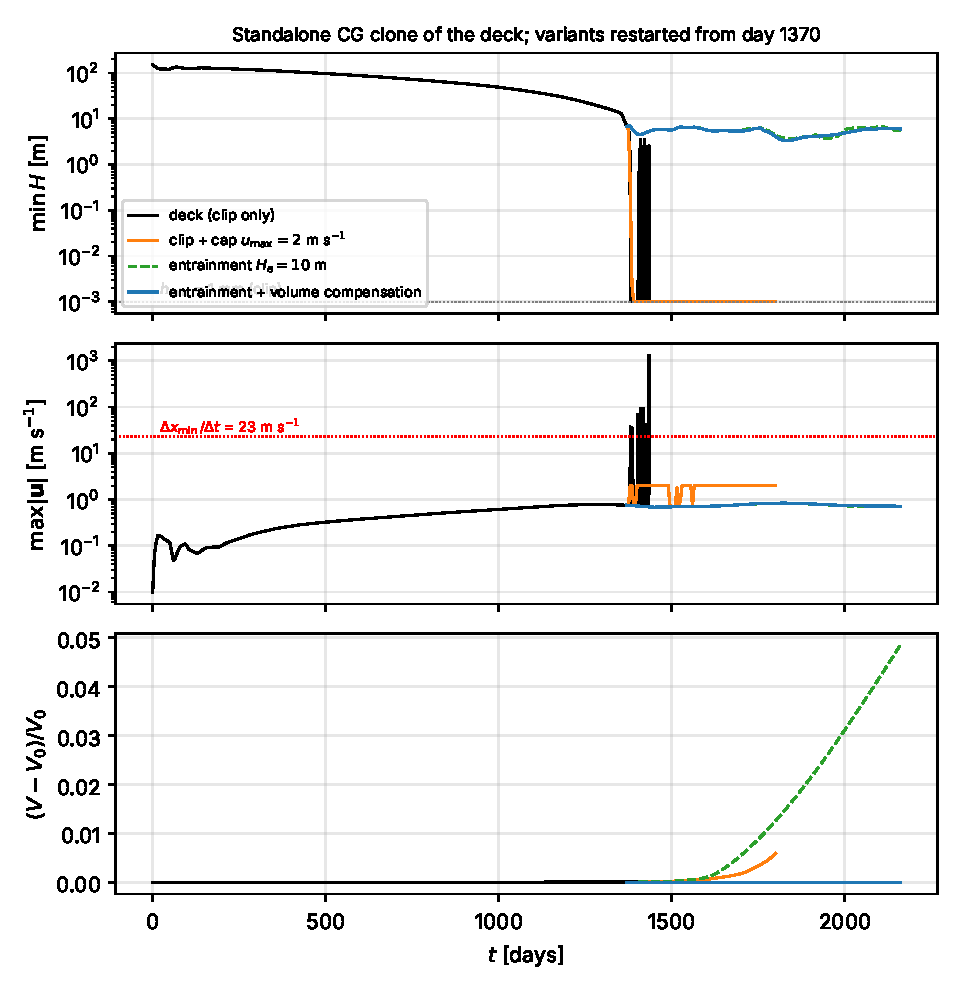
\includegraphics[width=0.72\textwidth]{ReducedGravity_thinlayers.pdf}
\caption{Standalone clone of the deck. Top: $\min H$; middle: $\max|\bu|$;
bottom: relative volume change. Black: deck (clip only); orange: clip and
cap; green dashed: entrainment without compensation; blue: entrainment with
volume compensation, the configuration of \code{ReducedGravity\_entrain}.}
\label{fig:runs}
\end{figure}

\paragraph{Deck switches.}
\code{:swe\_limiter => "clip"}, \code{:swe\_limiter\_schedule => "stage"},
\code{:swe\_hmin => 1e-3}, \code{:swe\_umax => 2.0} (safety net),
\code{:swe\_conserve\_volume => true}, \code{:lmass\_diagnostic => true};
$H_e$ and $t_e$ are \code{\_H\_ENTRAIN\_SWE} and \code{\_T\_ENTRAIN\_SWE} in
\code{user\_source.jl}.

\newpage
\section*{References}
\small
\begin{itemize}\setlength\itemsep{1pt}
\item B.-J. Choi, M. Iskandarani, J. Levin, D. B. Haidvogel (2004). A spectral
finite-volume method for the shallow water equations. \emph{Mon.\ Wea.\ Rev.}\
132, 1777--1791.
\item A. Kurganov, G. Petrova (2007). A second-order well-balanced positivity
preserving central-upwind scheme for the Saint-Venant system.
\emph{Commun.\ Math.\ Sci.}\ 5, 133--160.
\item S. Marras, M. A. Kopera, E. M. Constantinescu, J. Suckale,
F. X. Giraldo (2018). A residual-based shock capturing scheme for the
continuous/discontinuous spectral element solution of the 2D shallow water
equations. \emph{Adv.\ Water Resour.}\ 114, 45--63.
\item J. P. McCreary, P. K. Kundu (1988). A numerical investigation of the
Somali Current during the Southwest Monsoon. \emph{J.\ Mar.\ Res.}\ 46, 25--58.
\item A. T. Parsons (1969). A two-layer model of Gulf Stream separation.
\emph{J.\ Fluid Mech.}\ 39, 511--528.
\item H. Vandeven (1991). Family of spectral filters for discontinuous problems.
\emph{J.\ Sci.\ Comput.}\ 6, 159--192.
\item R. J. Spiteri, S. J. Ruuth (2002). A new class of optimal high-order
strong-stability-preserving time discretization methods.
\emph{SIAM J.\ Numer.\ Anal.}\ 40, 469--491.
\end{itemize}

\end{document}
